\documentclass[a4paper,14pt]{article}
\usepackage{blindtext}
\usepackage[T2A]{fontenc}
\usepackage[utf8]{inputenc}
\usepackage[english,russian]{babel}
\usepackage{listings}
\usepackage{geometry}
\usepackage{amssymb}
\usepackage{amsmath}
\usepackage[14pt]{extsizes}
\geometry{left=3cm}
\geometry{right=1.5cm}
\geometry{top=2cm}
\geometry{bottom=2cm}
\pagestyle{plain}
\usepackage{pgfplots}
\usepackage{filecontents}
\usepackage{graphicx}
\usepackage{indentfirst}
\DeclareGraphicsExtensions{.png}
\graphicspath{{images/}}
\usetikzlibrary{datavisualization}
\usetikzlibrary{datavisualization.formats.functions}
\usepackage{tabularx}
\pgfplotsset{width=7 cm}
\usepackage{xcolor}
%\renewcommand{\rmdefault}{ftm}
%\usepackage{mathptmx}
\usepackage{setspace}
%\usepackage{minted}
%\полуторный интервал
\onehalfspacing
\usepackage{colortbl}
\usepackage{tocloft}
\frenchspacing
\setcounter{page}{3}
\usepackage{multirow}
\usepackage{float}
\usepackage{multirow}

\renewcommand{\cftsecdotsep}{\cftdot}
\renewcommand{\cftsecleader}{\cftdotfill{\cftsecdotsep}}
\renewcommand{\cftsubsecleader}{\cftdotfill{\cftsecdotsep}}
\renewcommand{\cftsubsubsecleader}{\cftdotfill{\cftsecdotsep}}

%\renewcommand\cftchapdotsep{\cftdot}
%\renewcommand\cftsecdotsep{\cftdot}
%\renewcommand{\cftchapleader}{\cftdotfill{\cftchapdotsep}}

% Для измененных титулов глав:
% % подключаем нужные пакеты
%\definecolor{gray75}{gray}{0.75} % определяем цвет
%\newcommand{\hsp}{\hspace{20pt}} % длина линии в 20pt
% titleformat определяет стиль
%\titleformat{\chapter}[hang]{\Huge\bfseries}{\thechapter\hsp\textcolor{black}{|}\hsp}{0pt}{\Huge\bfseries}
%\usepackage{titlesec, blindtext, color}
%\titleformat{\chapter}[hang]{\Huge\bfseries}{\thechapter\hsp\textcolor{black}{|}\hsp}{0pt}{\Huge\bfseries}

% Для листинга кода:
\lstset{ %
extendedchars=\true,
inputencoding=utf8,
morekeywords={include, printf},
texcl=\true,
breaklines=\true,
escapeend=\end{russian},
escapechar=\%,
keepspaces=\true,
language=c,                 % выбор языка для подсветки
basicstyle=\small\sffamily, % размер и начертание шрифта для подсветки кода
numbers=left,               % где поставить нумерацию строк (слева\справа)
numberstyle=\tiny,           % размер шрифта для номеров строк
stepnumber=1,                   % размер шага между двумя номерами строк
numbersep=5pt,                % как далеко отстоят номера строк от подсвечиваемого кода
showspaces=\true,            % показывать или нет пробелы специальными отступами
showstringspaces=\true,      % показывать или нет пробелы в строках
showtabs=false,             % показывать или нет табуляцию в строках
frame=single,              % рисовать рамку вокруг кода
tabsize=4,                 % размер табуляции по умолчанию равен 2 пробелам
captionpos=t,              % позиция заголовка вверху [t] или внизу [b]
breaklines=true,           % автоматически переносить строки (да\нет)
breakatwhitespace=false, % переносить строки только если есть пробел
escapeinside={\//*}{*)}   % если нужно добавить комментарии в коде
}



\begin{document}

\begin{titlepage}

    \begin{table}
        \centering
        \footnotesize
        \begin{tabular}{cc}
            \multirow{8}{*}{
\includegraphics[scale=0.35]{bmstu.jpg}}
             &                                                                           \\
             &                                                                           \\
             & \textbf{Министерство науки и высшего образования Российской Федерации}    \\
             & \textbf{Федеральное государственное бюджетное образовательное учреждение} \\
             & \textbf{высшего образования}                                              \\
             & \textbf{<<Московский государственный технический}                         \\
             & \textbf{университет имени Н.Э. Баумана>>}                                 \\
             & \textbf{(МГТУ им. Н.Э. Баумана)}                                          \\
        \end{tabular}
    \end{table}

    \vspace{-2.5cm}

    \begin{flushleft}
        \rule[-1cm]{\textwidth}{3pt}
        \rule{\textwidth}{1pt}
    \end{flushleft}

    \begin{flushleft}
        ФАКУЛЬТЕТ Информатика и системы управления
    \end{flushleft}
    КАФЕДРА Программное обеспечение ЭВМ и информационные технологии

    \vspace{3cm}

    \begin{center}
        \textbf{Лабораторная работа № 6} \\
        \textbf{Дисциплина: <<Компьютерные сети>>}
        \vspace{0.5cm}
    \end{center}


    \vspace{3cm}

    \begin{flushleft}
        \begin{tabular}{ll}
            \textbf{Студент}       & Овчинникова А. П. \\
            \textbf{Группа}        & ИУ7-75Б           \\
            \textbf{Преподаватель} & Рогозин Н. О.     \\
        \end{tabular}
    \end{flushleft}

    \vspace{3cm}

    \begin{center}
        Москва, 2020 г.
    \end{center}

\end{titlepage}

\setcounter{page}{2}

Адрес локальной общей сети: 192.168.15.0/24.

Этот же адрес в двоичном формате (сетевая часть Ipv4 адреса отмечена \textcolor{blue}{синим}, хостовая часть Ipv4 адреса – \textcolor{red}{красным}):

\textcolor{blue}{1100 0000.1010 1000.0000 1111.}\textcolor{red}{0000 0000}

Маска:	1111 1111 .1111  1111.1111 1111.\textcolor{red}{0000 0000}

Начальный адрес сети: \textcolor{blue}{1100 0000.1010 1000.0000 1111.}\textcolor{red}{0000 0000} (192.168.15.0)

Широковещательный адрес: \textcolor{blue}{1100 0000.1010 1000.0000 1111.}\textcolor{red}{1111 1111}

(192.168.15.255)

Разделим сеть на 5 подсетей.

\begin{enumerate}
	\item Подсеть 1 должна поддерживать до 25 устройств.
	\item Подсеть 2 должна поддерживать до 5 устройств.
	\item Подсеть 3 должна поддерживать только 2 устройства.
	\item Подсеть 4 должна поддерживать до 5 устройств.
	\item Подсеть 5 должна поддерживать до 25 устройств.
\end{enumerate}


\textbf{Подсеть 1}

Вначале выделим адрес для подсети 1.

$2^5$ обеспечивает минимум 32 хоста - 2 адреса (начальный адрес сети и широковещательный адрес).

Начальный адрес подсети 1: 

192.168.15.0

Маска подсети 1:

1111 1111.1111 1111.1111 1111.1110 0000

(255.255.255.224)

Широковещательный адрес подсети 1:

192.168.15.31

Начальный адрес подсети 1 в CIDR-нотации:

192.168.15.0/27

\textbf{Подсеть 5}

Выделим адрес для подсети 5.

$2^5$ обеспечивает минимум 32 хоста - 2 адреса (начальный адрес сети и широковещательный адрес).


Начальный адрес подсети 5: 

192.168.15.32

Маска подсети 5:

1111 1111.1111 1111.1111 1111.1110 0000

(255.255.255.224)

Широковещательный адрес подсети 5:

192.168.15.63

Начальный адрес подсети 1 в CIDR-нотации:

192.168.15.32/27


\textbf{Подсеть 2}

Выделим адрес для подсети 2.

$2^3$ обеспечивает минимум 8 хостов - 2 адреса (начальный адрес сети и широковещательный адрес).


Начальный адрес подсети 2: 

192.168.15.64

Маска подсети 2:

1111 1111.1111 1111.1111 1111.1111 1000

(255.255.255.248)

Широковещательный адрес подсети 2:

192.168.15.71

Начальный адрес подсети 2 в CIDR-нотации:

192.168.15.64/29

\textbf{Подсеть 4}

Выделим адрес для подсети 4.

$2^3$ обеспечивает минимум 8 хостов - 2 адреса (начальный адрес сети и широковещательный адрес).


Начальный адрес подсети 4: 

192.168.15.72

Маска подсети 4:

1111 1111.1111 1111.1111 1111.1111 1000

(255.255.255.248)

Широковещательный адрес подсети 4:

192.168.15.79

Начальный адрес подсети 2 в CIDR-нотации:

192.168.15.72/29

\textbf{Подсеть 3}

Выделим адрес для подсети 3.

$2^2$ обеспечивает минимум 8 хостов - 2 адреса (начальный адрес сети и широковещательный адрес).


Начальный адрес подсети 3: 

192.168.15.80

Маска подсети 3:

1111 1111.1111 1111.1111 1111.1111 1100

(255.255.255.252)

Широковещательный адрес подсети 3:

192.168.15.83

Начальный адрес подсети 2 в CIDR-нотации:

192.168.15.80/30

\textbf{Настройка DHCP-серверов в Cisco Packet Tracer}

На рисунке \ref{fig:pc11} представлена конфигурация компьютера 1 из подсети 1. DHCP назначил ему IP адрес 192.168.15.4.

\newpage
\begin{figure}[!h]
   \center{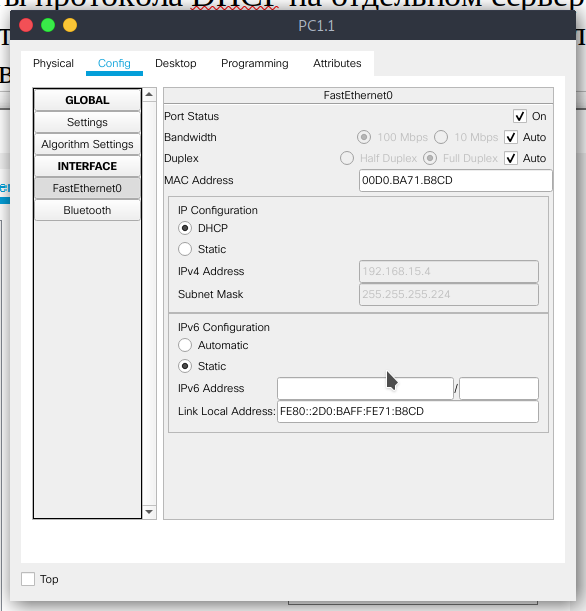
\includegraphics[width=15cm]{pc11}}
    \caption{Компьюетр в подсети 1.}
    \label{fig:pc11}
\end{figure}

\newpage
На рисунке \ref{fig:pc11ping} показано, что другой компьютер из подсети 1 с IP адресом 192.168.15.3 пингуется с компьютера 1 в подсети 1.

\begin{figure}[!h]
    \center{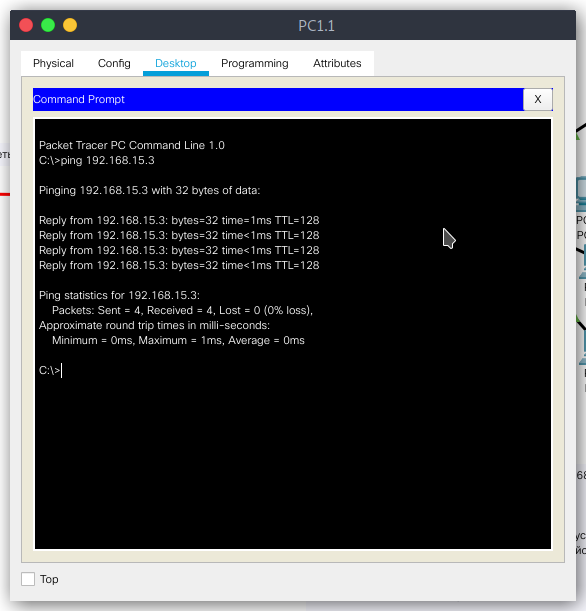
\includegraphics[width=15cm]{pc11ping}}
     \caption{Компьюетр в подсети 1 связывается с другим компьютером в этой же подсети.}
     \label{fig:pc11ping}
 \end{figure}

 \newpage

На рисунке \ref{fig:dhcps} представлена конфигурация DHCP-сервера.

 \begin{figure}[!h]
    \center{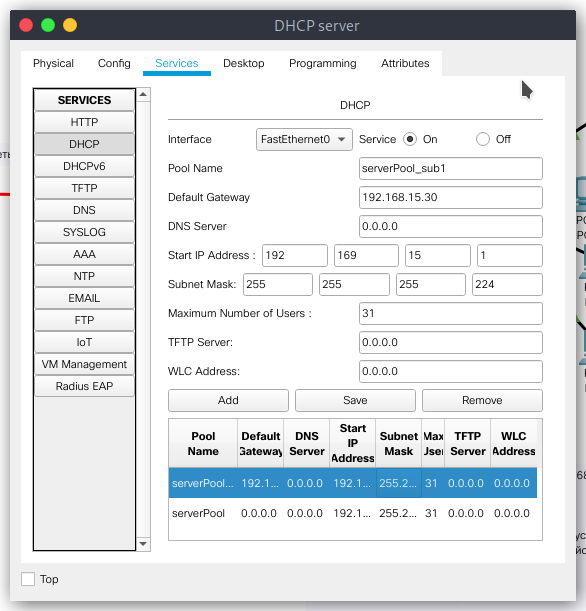
\includegraphics[width=15cm]{dhcps}}
     \caption{DHCP-сервер.}
     \label{fig:dhcps}
 \end{figure}

 \newpage

 Серверам из подсети 2 необходимо назначить статический адрес:

 \begin{figure}[!h]
    \center{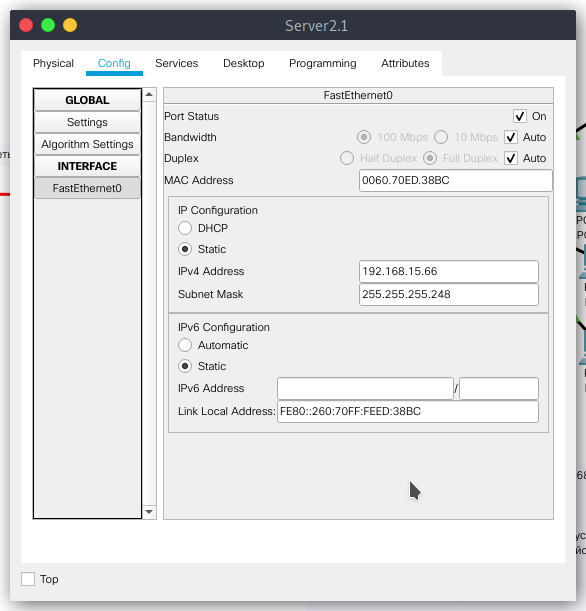
\includegraphics[width=15cm]{s21}}
     \caption{Сервер 1 из подсети 2.}
     \label{fig:s21}
 \end{figure}

 \newpage
 На рисунке \ref{fig:s21ping} показано, что сервер 1 из подсети 2 может связываться с другими серверами из этой же подсети.

 \begin{figure}[!h]
    \center{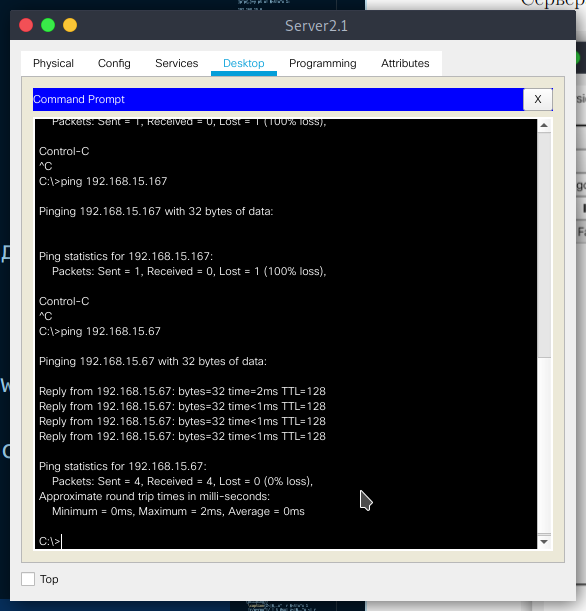
\includegraphics[width=15cm]{s21ping}}
     \caption{Сервер 1 из подсети 2 связывается с другим сервером.}
     \label{fig:s21ping}
 \end{figure}

 \newpage
 Последовательность команд для настройки роутера 1 как DHCP сервера для подсети 2:

 \begin{enumerate}
     \item conf t
     \item ip dhcp excluded-address 192.168.15.65 192.168.15.68
     \item ip dhcp pool pool\_sub2
     \item network 192.168.15.64 255.255.255.248
     \item default-router 192.168.15.65
     \item exit
     \item interface GigabitEthernet0/0/1
     \item ip address 192.168.15.65 255.255.255.248
     \item no shutdown
     \item exit
     \item exit
 \end{enumerate}

 \newpage

Настройка кабеля Serial 0/0/1 для роутера 1 представлена на рисунке \ref{fig:r1}.

\begin{figure}[!h]
    \center{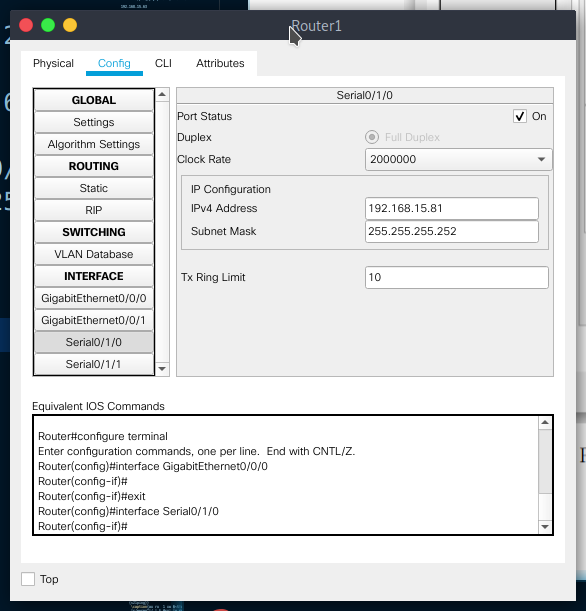
\includegraphics[width=15cm]{p1}}
    \caption{Роутер 1.}
    \label{fig:r1}
\end{figure}

\newpage

Остальные роутеры и подсети настраиваются аналогичным образом. Серверам в подсети 4 также назначены статические адреса.

На рисунке \ref{fig:pc51} показано, что роутер 2, работающий как DHCP-сервер для подсети 5, выдал компьютеру 1 из этой подсети адрес 192.168.15.34.

\begin{figure}[!h]
    \center{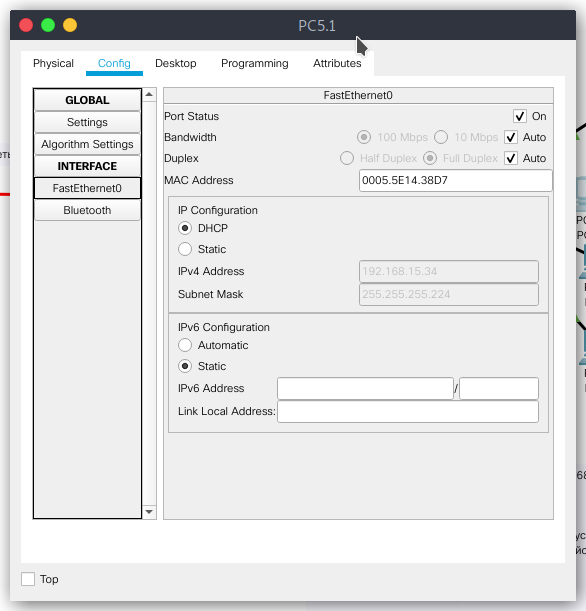
\includegraphics[width=15cm]{pc51}}
    \caption{Компьютер 1 из подсети 5.}
    \label{fig:pc51}
\end{figure}

\newpage

На рисунке \ref{fig:pc51ping} показано, что компьютер 1 из подсети 5 связывается с другим компьютером из этой же подсети.

\begin{figure}[!h]
    \center{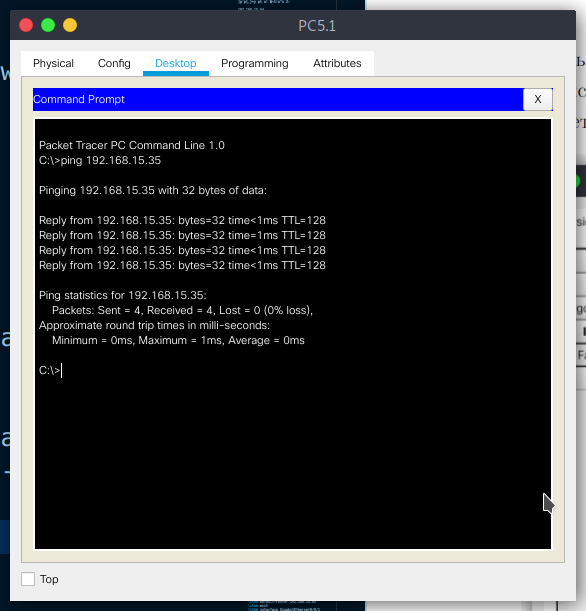
\includegraphics[width=15cm]{pc51ping}}
    \caption{Компьютер 1 из подсети 5 связывается с другим компьютером из этой подсети.}
    \label{fig:pc51ping}
\end{figure}

\end{document}
